\documentclass[12pt]{article}
\usepackage{amssymb,mathtools}
\usepackage[margin=1in]{geometry}
\usepackage{fancyhdr}
\usepackage{circuitikz}
\usepackage{graphicx}
\graphicspath{ {./Figures/} }
\usepackage{amsmath}
\usepackage{ragged2e}
\usepackage{subcaption} 
\usepackage{float}
\usepackage{cancel}
\usepackage{siunitx}
\pagestyle{fancy}
\usepackage[shortlabels]{enumitem}
\usepackage{mathtools}
\newcommand*{\permcomb}[4][0mu]{{{}^{#3}\mkern#1#2_{#4}}}
\newcommand*{\Comb}[2]{{}^{#1}C_{#2}}%
\DeclarePairedDelimiter\ceil{\lceil}{\rceil}
\DeclarePairedDelimiter\floor{\lfloor}{\rfloor}
\setlength{\headheight}{15 pt}
\lhead{Georgy Antonov}
\chead{HW 3}
\rhead{Neural Dynamics}

\begin{document}\noindent


\noindent\textbf{Question 1. Branching}
\begin{enumerate}
    \item[1.0] For the killed end (Dirichlet) boundary condition, we have
    $$R_{in} =  R_{\infty} \text{tanh}(L)$$
    where $R_{\infty}$ is the input resistance for a semi-infinite cable given by
    $$R_{\infty} = \sqrt{\frac{4\tilde{r}_{m}\tilde{r}_{a}}{\pi^{2}d^{3}}}$$
    and L is the electrotonic length given by 
    $$L = \frac{l}{\lambda}$$
    where $\lambda$ is the length constant defined as
    $$\lambda = \sqrt{\frac{\tilde{r}_{m}d}{4\tilde{r}_{a}}}$$
    $\tilde{r}_{m}$ and $\tilde{r}_{a}$ are the specific membrane and axial resistances, respectively. Hence, for the input resistance for compartment 2 we have
    $$R_{in,2} = \sqrt{\frac{4\cdot 1\cdot 1}{\pi^{2}\left(5\cdot 10^{-6}\right)^{3}}}\cdot \text{tanh}\left(0.089\right) = 5.05 \, \text{M\si{\ohm}}$$
    For the sealed end (Neumann) boundary condition we have
    $$R_{in} =  R_{\infty} \text{coth}(L)$$
    Acccordingly, for compartment 3 we have
    $$R_{in,3} = \sqrt{\frac{4\cdot 1\cdot 1}{\pi^{2}\left(4\cdot 10^{-6}\right)^{3}}}\cdot \text{coth}\left(0.1\right) = 798.45 \, \text{M\si{\ohm}}$$
    Note the following relationship
    $$R_{L,1}^{-1} = \left(R_{in,2}^{-1} + R_{in,3}^{-1}\right)$$
    Therefore, the leak resistance for compartment 1 is
    $$R_{L,1} = \left(\left(5.05\cdot 10^{6}\right)^{-1} + \left(798.45\cdot 10^{6}\right)^{-1}\right)^{-1} = 5.02 \, \mu \text{\si{\ohm}}$$
    \item[1.1] To compute the potential $V(\infty)$ in response to constant current $I_{0}=1 \, \text{nA}$ we need to assume that the system has relaxed to a stationary solution and apply the formula for a finite cable potential as shown below
    $$V(X) = E_{m} + R_{\infty}I_{0}\frac{R_{L}\text{cosh}\left(L-X\right) + R_{\infty}\text{sinh}\left(L-X\right)}{R_{L}\text{sinh}\left(L\right) + R_{\infty}\text{cosh}\left(L\right)}$$
    where $R_{\infty}$ for compartment 1 is computed as shown above and X is defined as 
    $$X = \frac{x}{\lambda}$$
    where x is the distance along the compartment. Thus, plugging in the numbers and setting $t=\infty$ and $x=0$ gives
    $$X(\infty) = 6.388 \, \text{mV}$$
    From this we can compute the input resistance $R_{in, 1}$
    $$R_{in, 1} = \frac{6.338\cdot 10^{-3}}{10^{-9}} = 6.388 \, \text{M \si{\ohm}}$$
    \item[1.2] To get the current entering compartments 2 \& 3, $I_{L}$, we compute
    $$V(X=L) = E_{m} + R_{\infty}I_{0}\frac{R_{L}\text{cosh}\left(0\right) + R_{\infty}\text{sinh}\left(0\right)}{R_{L}\text{sinh}\left(L\right) + R_{\infty}\text{cosh}\left(L\right)} = 4.993\cdot 10^{-15} \, \text{A}$$
    And the corresponsing $I_L$ is then
    $$I_L = \frac{V(L)}{R_{L}} = 0.995 \, \text{nA}$$
    Then we apply the current divider formula for resistors connected in parallel
    $$I_{X} = \frac{R_{T}}{R_{X} + R_{T}}I_{T}$$
    Where $I_{X}$ is the current flowing through the resistor with resistance $R_{X}$, and $I_{T}$ and $R_{T}$ are the total current entering and the total resistance in parallel, respectively.
    Thus, by substituting the values we get\\
    $$I_{2} = 9.883 \, \text{nA} \; \text{, and} \; I_{3} = 0.0625 \, \text{nA}$$
    \item[1.3] Assuming that compartment 2 is terminated by a sealed end will change its input resistance and, consequently, the leak resistance for compartment 1. The new input resistance for compartment 2 is thus
    $$R_{in,2} = \sqrt{\frac{4\cdot 1\cdot 1}{\pi^{2}\left(5\cdot 10^{-6}\right)^{3}}}\cdot \text{coth}\left(0.089\right) = 641.46 \, \text{M\si{\ohm}}$$
    Hence, $R_{L, 1}$ becomes
    $$R_{L,1} = \left(\left(641.46\cdot 10^{6}\right)^{-1} + \left(798.45\cdot 10^{6}\right)^{-1}\right)^{-1} = 355.70 \, \text{M\si{\ohm}}$$
    And by applying the above formula for $V(\infty)$ we get 
    $$V(\infty) = 104 \, \text{mV}$$
\end{enumerate}

\noindent\textbf{Question 2. Equivalent Cylinder}
\begin{enumerate}
    \item[2.1] No, this branching model cannot be simplified by an equivalent cylinder model, for the branching compartments do not follow the 
    '3/2 diameter rule', which must satisfy 
    $$(d_{1})^{\frac{3}{2}} = (d_{2})^{\frac{3}{2}} + (d_{3})^{\frac{3}{2}}$$
    where $d_{1}$, $d_{2}$, and $d_{3}$ are the corresponding compartment diameters.
    \item[2.2] To find the required diameters, we can use the formula for electrotonic lenghts which must hold if we are to simplify this two-branch model.
    The formula appears below  
    $$L_{i} = \frac{l_{i}}{\lambda_{i}} = \frac{l_{j}}{\lambda_{j}} = L_{j} \quad \text{for} \; i, j > 1$$
    This can be simplified to (e.g for $i=2$ and $j=3$)
    \begin{align*}
        \frac{l_{2}}{\lambda_{2}} &= \frac{l_{3}}{\lambda_{3}}\\
        \implies \lambda_{3} &= \frac{l_{3}\lambda_{2}}{l_{2}}\\
        \implies \sqrt{d_{3}} &= \frac{l_{3}\sqrt{d_{2}}}{l_{2}}\\
        \implies d_{3} &= d_{2}\left(\frac{l_{3}}{l_{2}}\right)^{2}
    \end{align*}
    Hence, plugging in the numbers gives us
    $$d_{3} = 2.04 \, \mu \text{m}$$
    Then applying the '3/2 rule' gives us
    $$d_{1} = (d_{2}^{\frac{3}{2}} + d_{3}^{\frac{3}{2}})^{\frac{2}{3}} = 4.92 \, \mu \text{m}$$
    As regards the length and the diameter of the equivalent cylinder, the entire tree can be modelled by a single cylinder of 
    diameter $d_{1}$, length constant $\lambda_{1}$ and $l_{e} = (L_{1} + L_{D})\lambda_{1}$, where
    $L_{D} = L_{2} = L_{3}$. Thus,
    $$l_{e} = l_{1} + l_{2}\left(\sqrt{\frac{d_{1}}{d_{2}}}\right) = 415.3 \, \mu \text{m}$$
    \item[2.3] By applying the same two conditions as above, we have
    \begin{align*} 
    d_{3} &= d_{2}\left(\frac{l_{3}}{l_{2}}\right)^{2}\\
    d_{4} &= d_{2}\left(\frac{l_{4}}{l_{2}}\right)^{2} \qquad \text{(Generalisation of the 3/2 rule)}
    \end{align*}
    Hence, we arrive at
    \begin{align*}
        d_{1} &= d_{2}\left(1 + \left(\frac{l_{3}}{l_{2}}\right)^{3} + \left(\frac{l_{4}}{l_{2}}\right)^{3}\right)^{\frac{2}{3}}\\
        \implies d_{2} &= \frac{d_{1}}{\left(1 + \left(\frac{l_{3}}{l_{2}}\right)^{3} + \left(\frac{l_{4}}{l_{2}}\right)^{3}\right)^{\frac{2}{3}}}\\
        \implies d_{2} &= 10.78 \mu m\\
    \end{align*}
    We can now solve for the other diameters by the above formulae
    \begin{align*}
        d_{3} &= 10.78\left(\frac{100}{150}\right)^{2} = 4.79 \mu m\\
        d_{4} &= 10.78\left(\frac{120}{150}\right)^{2} = 6.90 \mu m\\
    \end{align*}
    The diameter of the equivalent cylinder will similarly be $d_{1}$ and the length can be determined as in 2.2
    $$l_{e} = l_{1} + l_{2}\left(\sqrt{\frac{d_{1}}{d_{2}}}\right) = 392.74 \, \mu \text{m}$$
\end{enumerate}

\noindent\textbf{Question 3. Simulation of a two-compartment model of the passive membrane}
\begin{enumerate}
\item[3.1]
\begin{figure}[h]
    \centering
    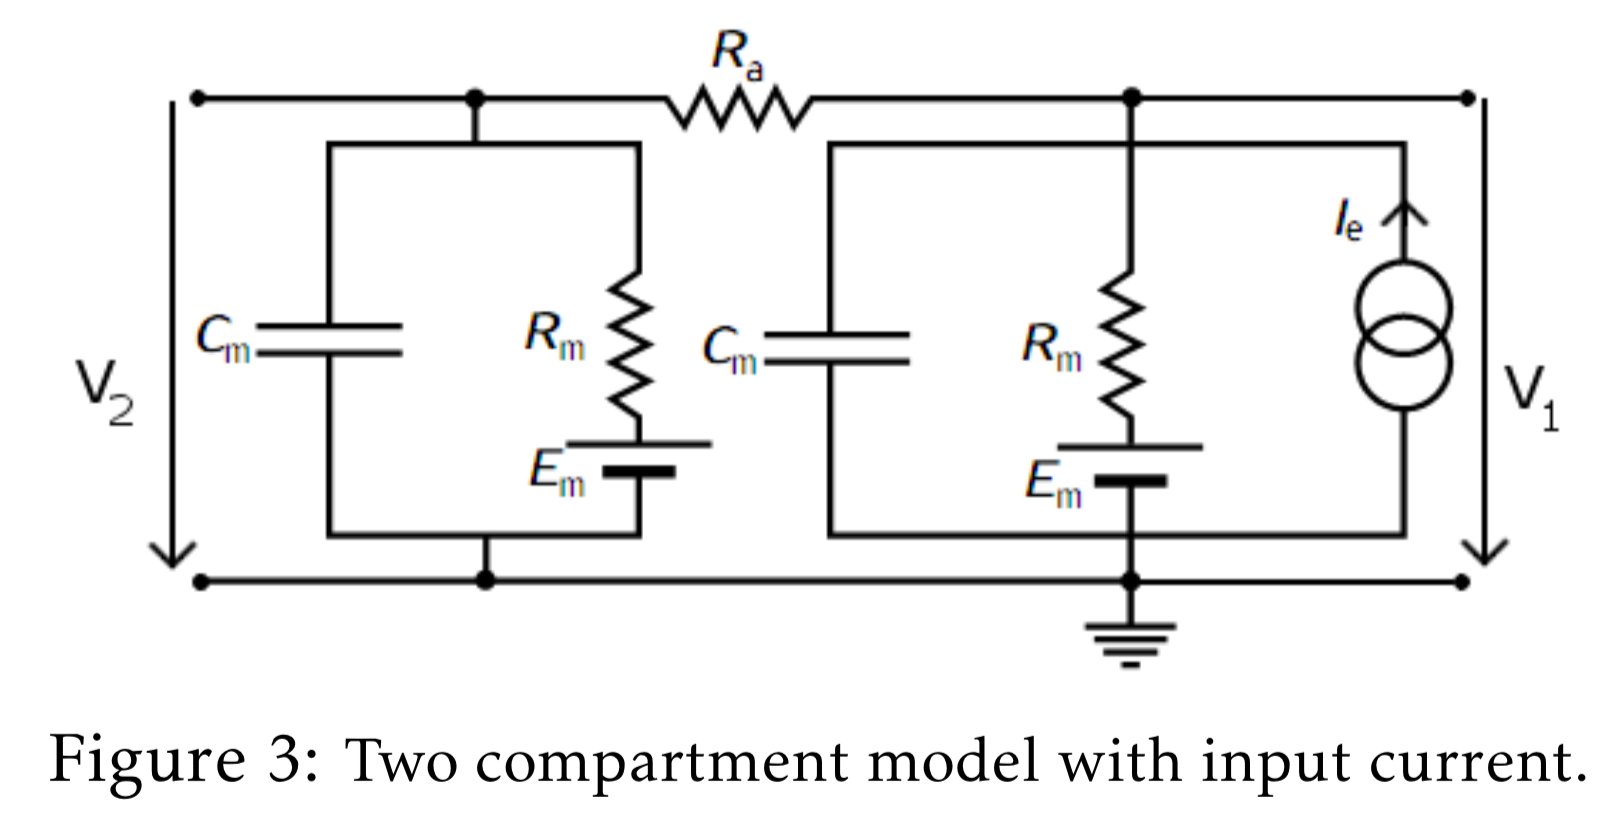
\includegraphics[width=0.7\textwidth]{circuit.png}
\end{figure}
According to the Kirchoff's law, total current leaving a node must be equal to total current entering that node. For the compartment 
on the left hand side (let us call it compartment 2), we have 
\begin{align*}
    \frac{V_{1}(t) - V_{2}(t)}{R_{a}} &= C_{m}\frac{dV_{2}(t)}{dt} + \frac{V_{2}(t)-E_{m}}{R_m}\\
    \implies C_{m}\frac{dV_{2}(t)}{dt} &= \frac{V_{1}(t) - V_{2}(t)}{R_{a}} + \frac{E_{m} - V_{2}(t)}{R_m}\\
    \implies \frac{dV_{2}(t)}{dt} &= \frac{V_{1}(t) - V_{2}(t)}{R_{a}C_{m}} + \frac{E_{m} - V_{2}(t)}{\tau_{m}}\\
\end{align*}
Similarly, for compartment 1 we have
\begin{align*}
    I_{e}(t) &= C_{m}\frac{dV_{1}(t)}{dt} + \frac{V_{1}(t)-E_{m}}{R_m} + \frac{V_{1}(t) - V_{2}(t)}{R_{a}}\\
    \implies C_{m}\frac{dV_{1}(t)}{dt} &= \frac{E_{m} - V_{1}(t)}{R_m} + \frac{V_{2}(t) - V_{1}(t)}{R_{a}} + I_{e}(t)\\
    \implies \frac{dV_{1}(t)}{dt} &= \frac{E_{m} - V_{1}(t)}{\tau_{m}} + \frac{V_{2}(t) - V_{1}(t)}{R_{a}C_{m}} + I_{e}(t)\frac{1}{C_{m}}\\
\end{align*}
We can now approximate both with the forward Euler method 
$$\frac{dV}{dt} \approx \frac{V(t+\Delta t)-V(t)}{\Delta t}$$
Hence, solving for both $V_{1}(t + \Delta t)$ and $V_{2}(t + \Delta t)$ we get
\begin{align*}
    V_{1}(t+\Delta t) &=  V_{1}(t) + \Delta t\left(\frac{E_{m} - V_{1}(t)}{\tau_{m}} + \frac{V_{2}(t) - V_{1}(t)}{R_{a}C_{m}} + I_{e}(t)\frac{1}{C_{m}}\right)\\
    V_{2}(t+\Delta t) &=  V_{2}(t) + \Delta t\left(\frac{V_{1}(t) - V_{2}(t)}{R_{a}C_{m}} + \frac{E_{m} - V_{2}(t)}{\tau_{m}}\right)\\
\end{align*}
\item[3.2] Next, I simulated the response of this two-compartment model to the current 
\[
    I_{e}(t)= 
\begin{cases}
    0, & t < t_{e}\\
    -100 \, \text{pA} ,              & t_{e} \leqslant t < t_{s}\\
    0, & t_{s} \leqslant t\\
\end{cases}
\]
where $t_{e} = 0.4 \, \text{s}$ and $t_{s} = 0.44 \, \text{s}$ with $E_{m} = 0 \, \text{V}$, $R_{m} = 265 \, \text{M\si{\ohm}}$, $R_{a} = 7 \, \text{M\si{\ohm}}$. I also 
assumed that the initial conditions were $V_{1}(t) = 0$ and $V_{2}(t) = 0$. 
The results appear in Figure 1.
\begin{figure}[h]
    \centering
    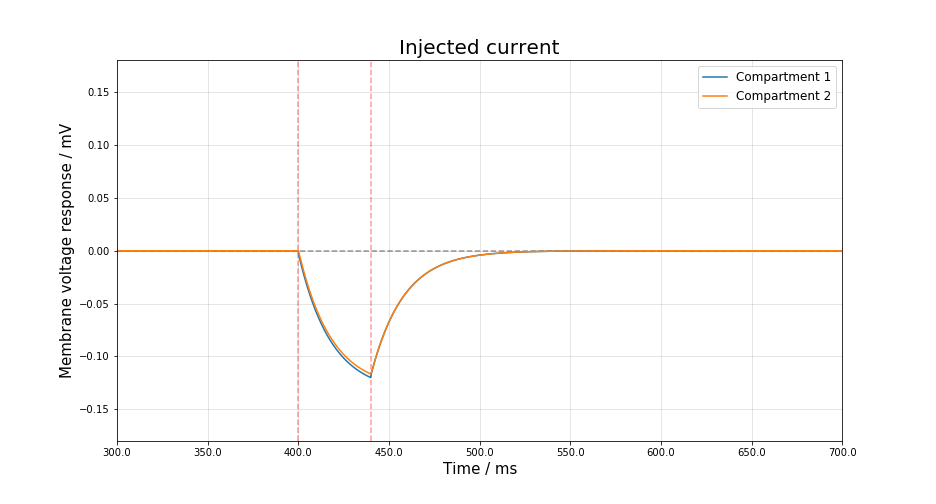
\includegraphics[width=\textwidth]{Ra_7M.png}
    \caption{Voltage resposes for compartments 1 and 2 with $R_{a} = 7 \, \text{M\si{\ohm}}$.}
\end{figure}
Wtih increasing the axial resistance, $R_{a}$, the 'responsiveness' of compartment 2 gradually decreased, as
can be seen in Figures 2 and 3.
\begin{figure}[h]
    \centering
    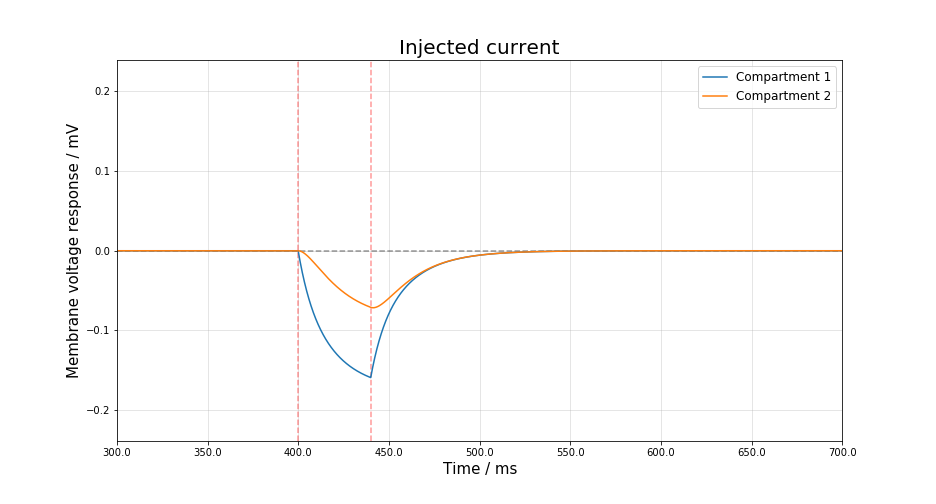
\includegraphics[width=\textwidth]{Ra_265M.png}
    \caption{Voltage resposes for compartments 1 and 2 with $R_{a} = 265 \, \text{M\si{\ohm}}$.}
\end{figure}
\begin{figure}[h]
    \centering
    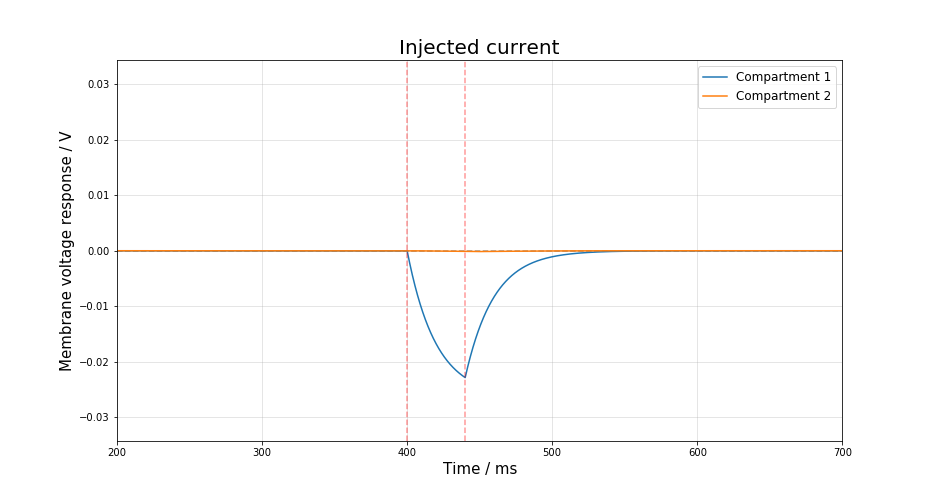
\includegraphics[width=\textwidth]{Ra_30G.png}
    \caption{Voltage resposes for compartments 1 and 2 with $R_{a} = 30 \, \text{G\si{\ohm}}$.}
\end{figure}
Figure 3 shows voltage responses at $R_{a} = 30 \, \text{G\si{\ohm}}$. In this case, compartment 2 has no response at all,
for the axial resistance is so high the current hardly ever reaches it.
\item[3.3] Finally, the model was simulated for 2 seconds with injected sinusoid current $I_{e}(t) = 100\text{pAsin}(2\pi ft)$ having 
all the parameters as before and $R_{a} = 300 \, \text{M\si{\ohm}}$. An example response for $f=20 \, \text{Hz}$ is shown in Figure 4 
and the resultant Bode diagram for a range of frequencies appears in Figure 5. Amplitudes for the bode diagram were conputed after 1s of stimulation to 
ensure the voltages have relaxed to sinusoidal output.
\begin{figure}[h]
    \centering
    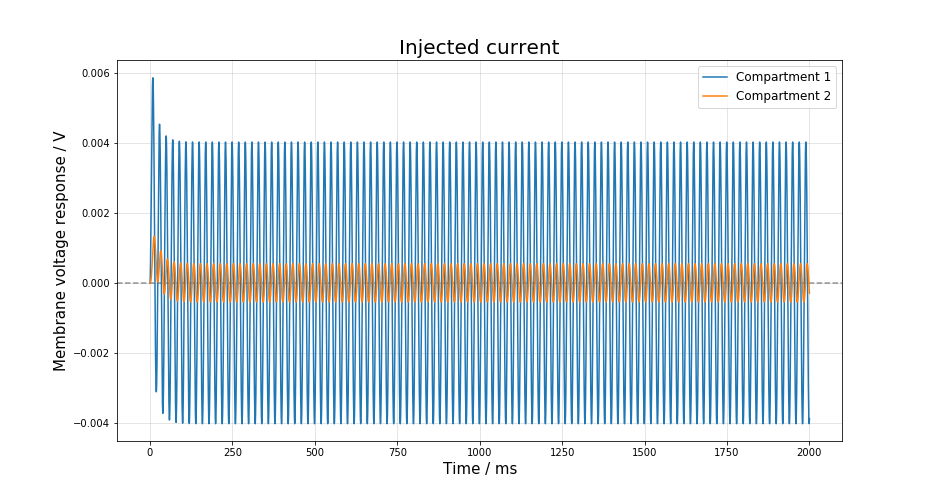
\includegraphics[width=\textwidth]{Sin_Ra_300M.png}
    \caption{Voltage resposes for compartments 1 and 2 for a sinusoid current.}
\end{figure}
\begin{figure}[h]
    \centering
    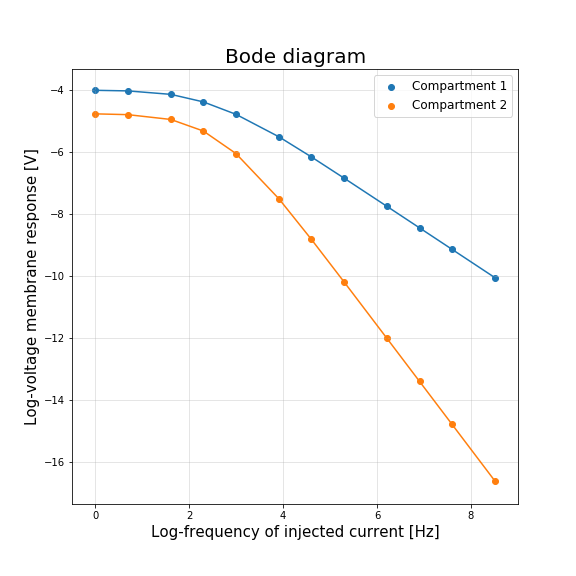
\includegraphics[width=\textwidth]{Bode.png}
    \caption{Stationary log-voltage resposes (after 1s) for compartments 1 and 2 for different log-frequencies of the injected current.}
\end{figure}
\end{enumerate}
\end{document}
